% chapter two: xenon1t

\chapter{The XENON1T Experiment}

The leading WIMP direct detection experiment is run by the XENON collaboration, of which XENON1T is the latest version of a series of ever-larger detectors~\cite{Angle:2007uj,Aprile:2011dd}. Built in central Italy at Laboratori Nazionali del Gran Sasso (LNGS), XENON1T is the largest and most sensitive xenon dual-phase time projection chamber (TPC) in the world at the time of commisioning, containing over $3200\1{kg}$ of xenon and a fiducial mass exceeding $1000\1{kg}$~\cite{Aprile:2017iyp}.

\section{Operational Overview}

The operation of a dual-phase TPC is as follows. When something interacts with an atom (xenon, argon, etc) inside the detector, it will produce prompt scintillation from the deexcitation of atoms involved, and liberated electrons. These photons provide what is called the \textit{S1} or \textit{prompt} signal, and is measured by arrays of Hamamatsu R11410-21 photomultipler tubes (PMTs)~\cite{Aprile:2015lha} above and below the target. An external electrical field drifts these electrons towards the liquid surface, where a second, much stronger electric field accelerates the electrons into the lower-density gas. These energetic electrons will interact with the gas, creating more light that is again collected by the PMT arrays. This signal is variably called the \textit{S2}, \textit{delayed}, or \textit{ionization} signal. The time difference between the S1 and S2 is the amount of time the electrons were drifing, and yields the depth or $z$ coordinate of the interaction. The hit pattern on the top PMT array yields the $(x,y)$ position of the event, as the PMTs directly above the S2 location will see more photons and produce a stronger signal. Figure~\ref{fig:idealized_event} shows schematically a typical event.

\begin{figure}[htb]
	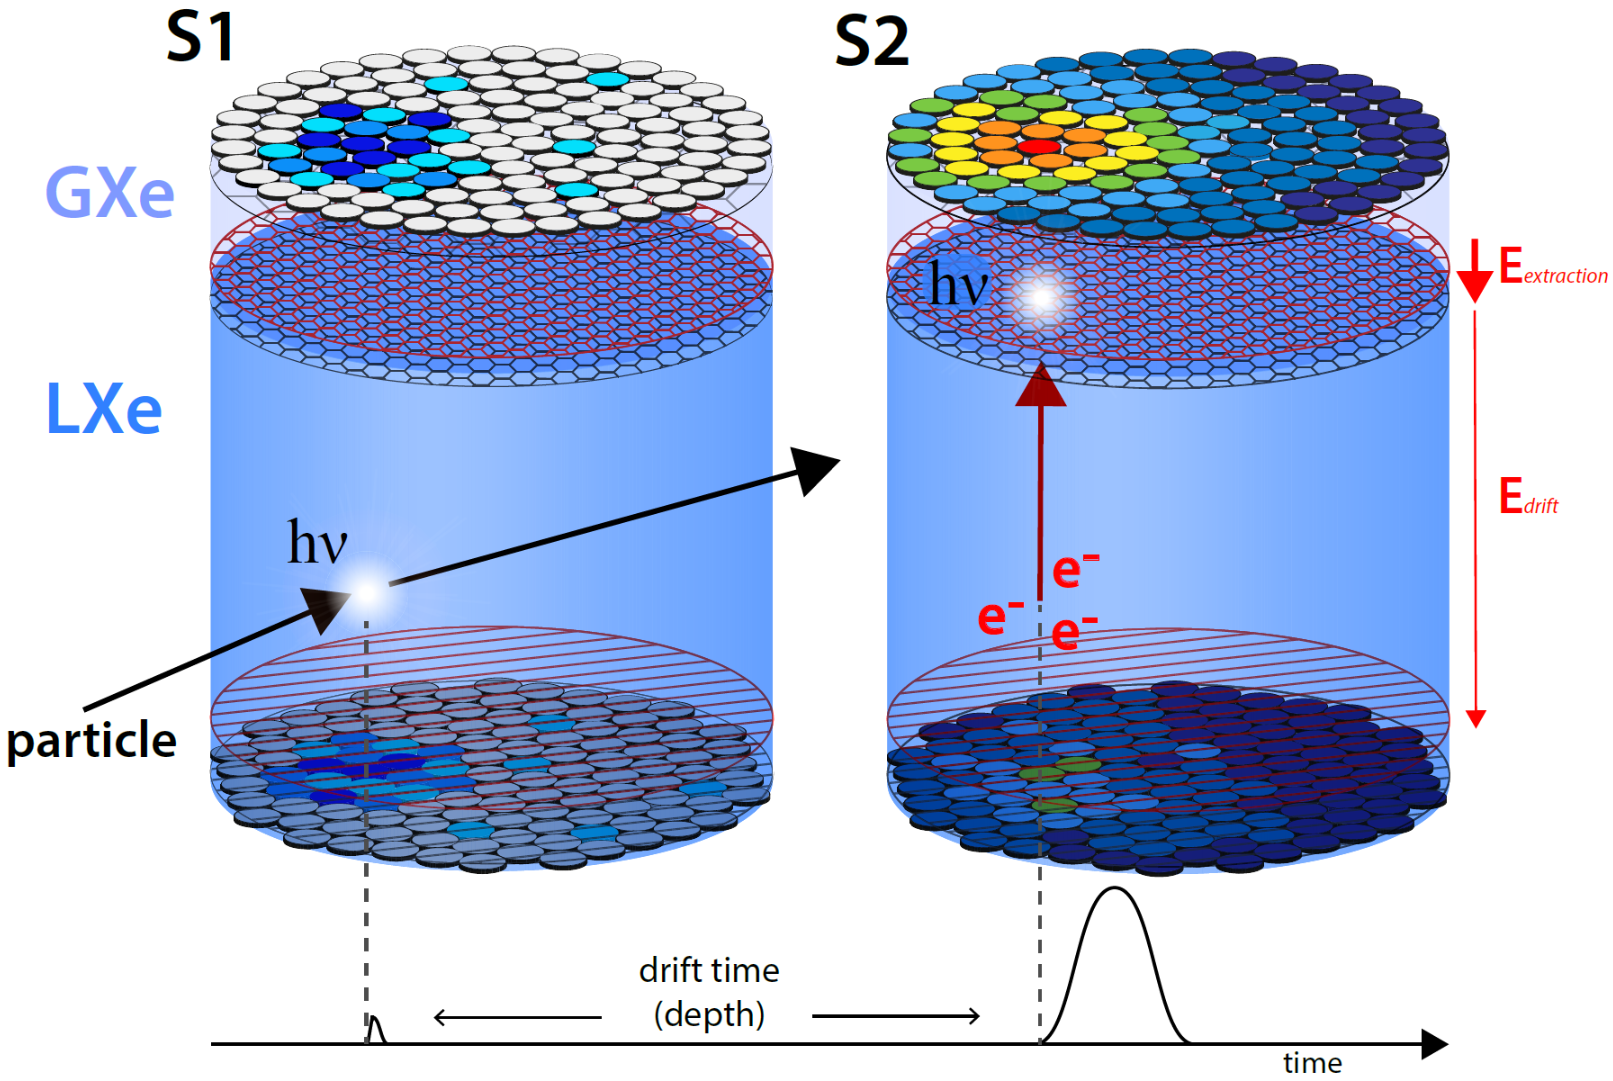
\includegraphics[width=\textwidth]{figures/xe1t/tpc_xe1t_workingprinciple_v2}
	\caption{An idealized event inside a dual-phase TPC. An interaction in the liquid produces both prompt scintillation (\textit{S1}) and quasi-free electrons. Under the influence of an applied electric field, these electrons drift toward the liquid surface, where a second, stronger electric field extracts the electrons into the gas. This causes energetic collisions with the gasseous atoms, resuling in delayed scintillation (\textit{S2}).}\label{fig:idealized_event}
\end{figure}

\section{System Overview}

The XENON1T detector is composed of numerous subsystems, which will be discussed here in some detail.

\subsection{Water tank}

The detector is housed in the center of a large tank of high-purity water, $10\1{m}$ in diameter and $10\1{m}$ in height. While the rock overburden at LNGS reduces the cosmogenic muon flux to about 1 per square meter per hour~\cite{Bellini:2012te}, these muons typically have extremely high energies and take a long time to fully dissipate all their energy. Thus, muons can still regularly traverse the detector volume. However, by surrounding the detector with water, the resulting Cherenkov radiation produced when muons traverse this water can be detected by an array of PMTs placed in the water, and a coincident event in the TPC itself tagged~\cite{Aprile:2014zvw}.

Furthermore, the water also acts to shield the TPC from radioactivity in the surrounding rock. The trigger rate in the detector decreases significantly as the tank is filled, as shown in Figure~\ref{fig:waterlevel}.

\begin{figure}[htb]
    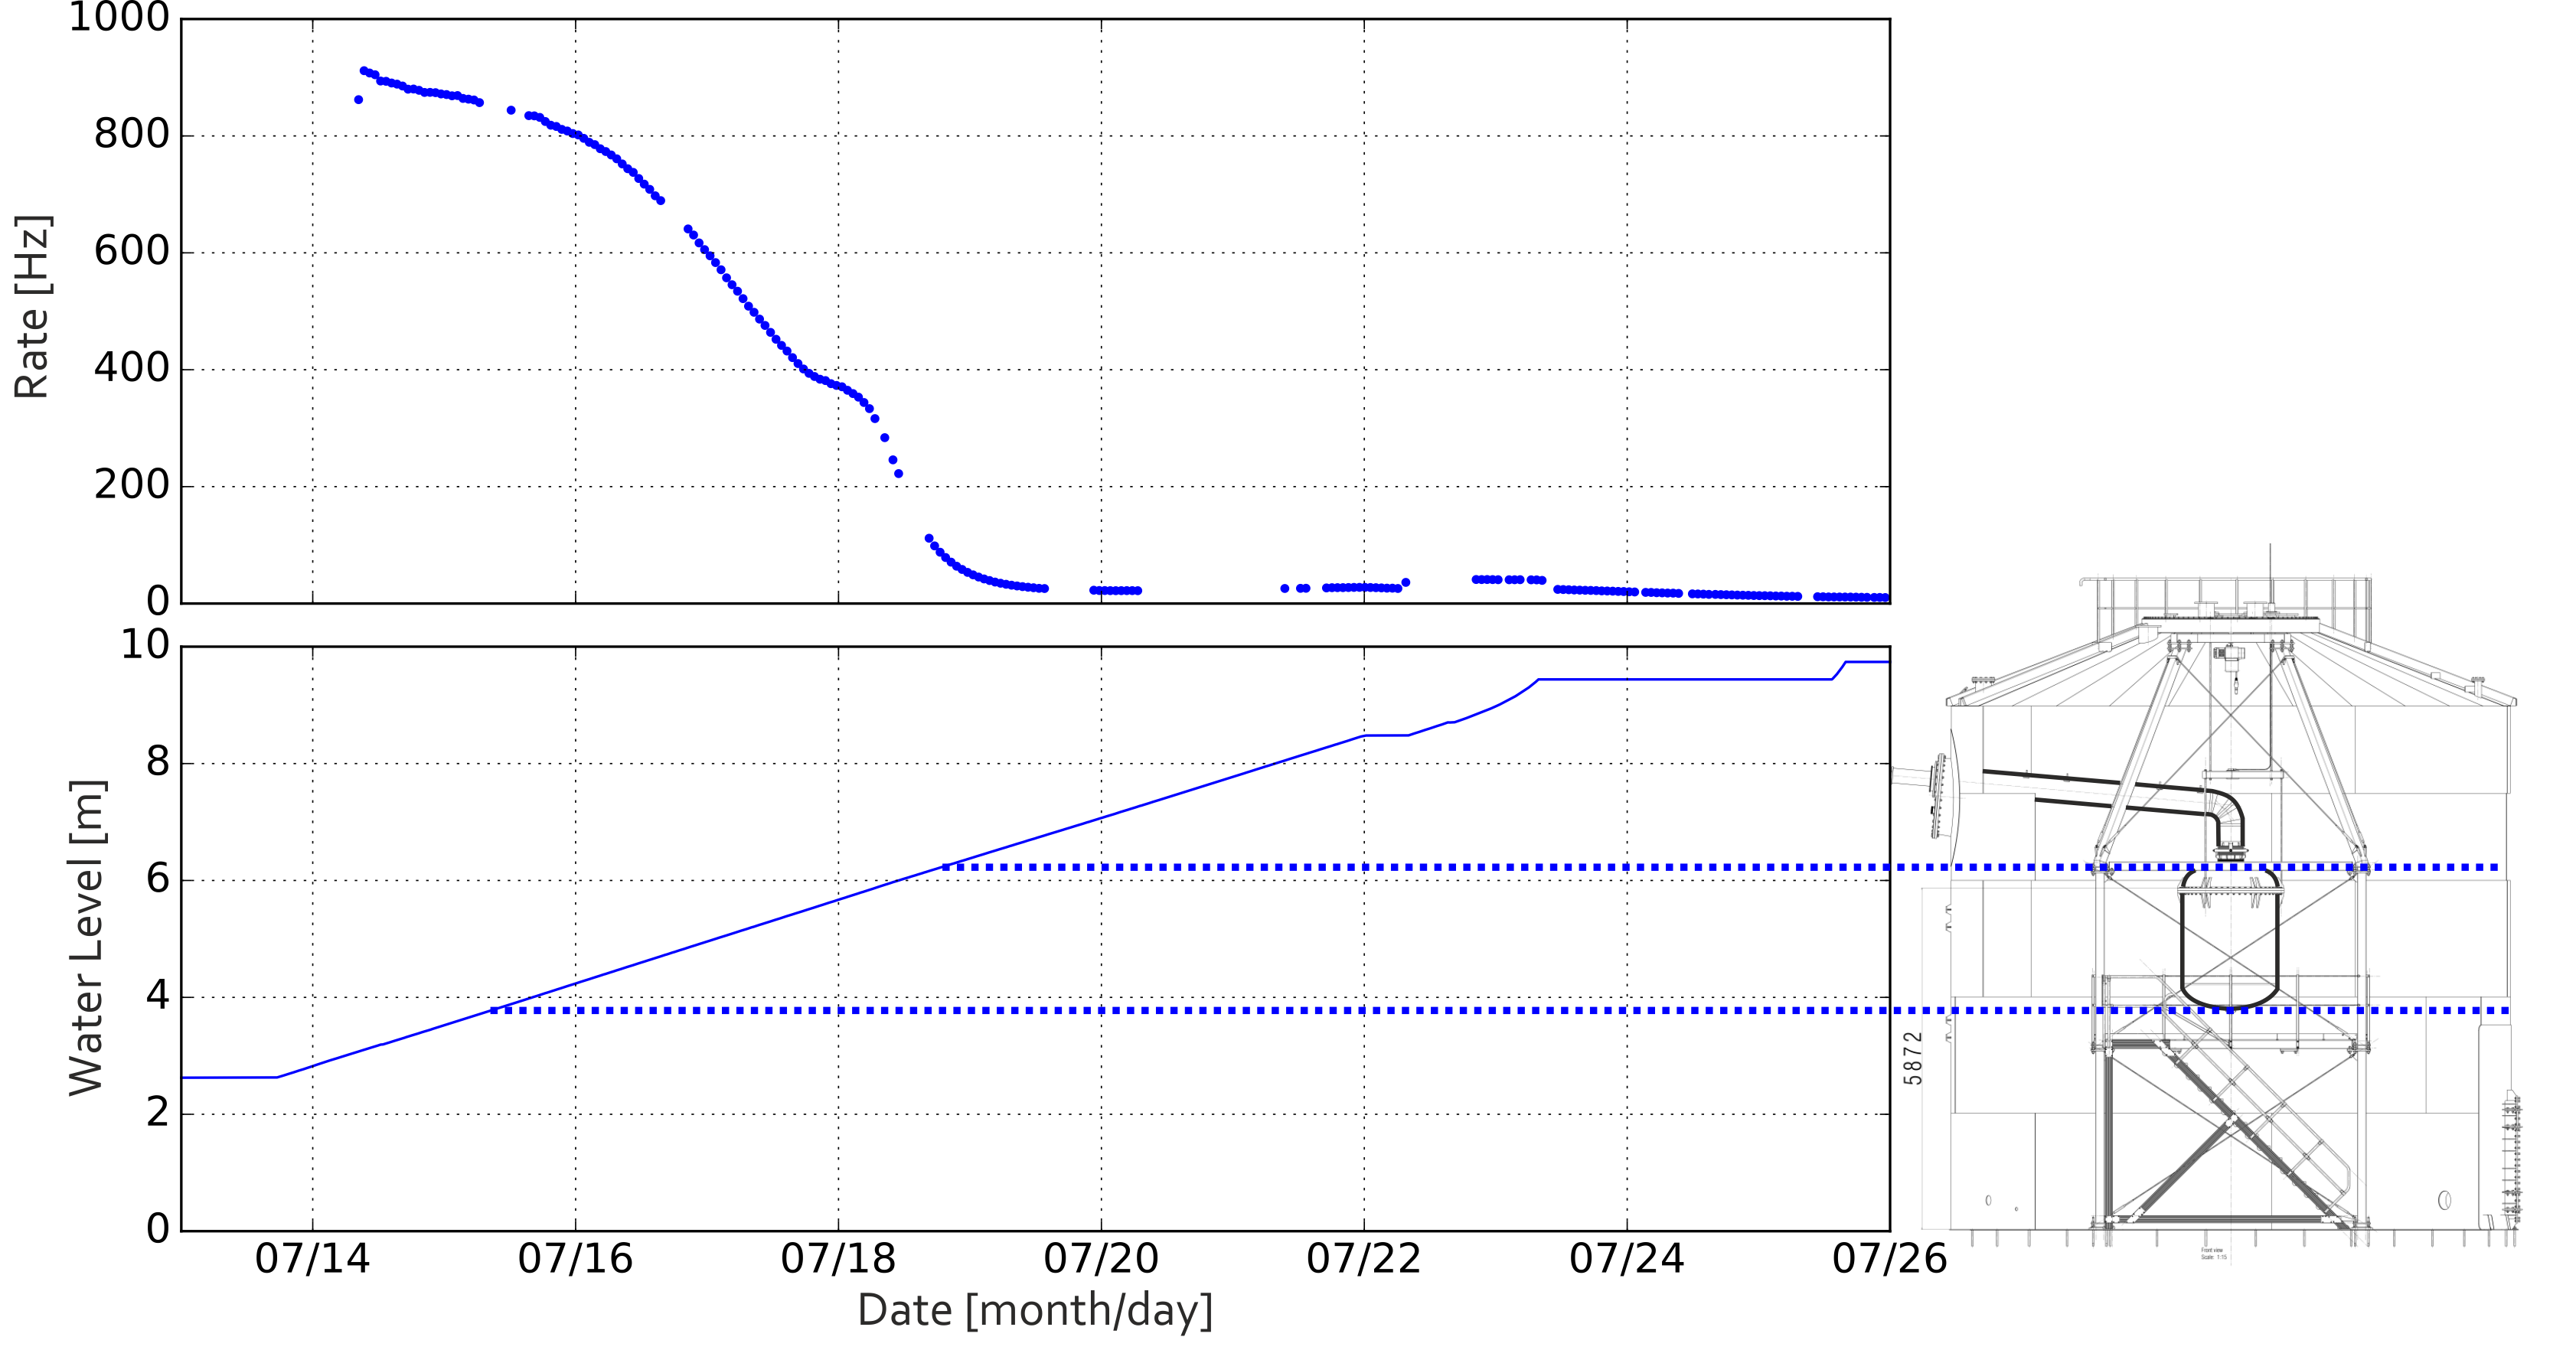
\includegraphics[width=\textwidth]{figures/xe1t/water_level_part_2}
    \caption{The trigger rate in XENON1T during the filling of the water tank. Surrounding the detector with several meters of water provides a reduction in trigger rate by two orders of magnitude.}\label{fig:waterlevel}.
\end{figure}

Additionally, in the center of the tank stands the support structure, which holds the cryostat as well as the temporary platform which can be erected for the purposes of performing maintenance on the TPC, cryostat, or surrounding systems.

\subsection{External calibration systems}

XENON1T has two primary external calibration systems. The first are known as the belt systems, and provide the ability to position radioactive sources at various locations surrounding the cryostat. The second is the deuterium-deuterium plasma fusion neutron generator~\cite{Lang:2017ymt}.

\subsubsection{Belt systems}

Three systems of belts are mounted in the water tank. Two of these systems have purely vertical travel (I-belts), and the third is capable of moving a source all the way underneath the detector along a secant (U-belt). These are located as shown in Figure~\ref{fig:belts}.

\begin{figure}[htb]
    \begin{center}
    \includegraphics[width=\textwidth]{figures/xe1t/cryo_belts_ng_colored}
    \end{center}
    \caption{Placement of external calibration systems around the XENON1T cryostat. The neutron generator (green) is used for nuclear recoil calibrations, while the I-belts (blue) and U-belt (red) allow for the positioning of $\gamma$ sources to measure (amonst other things) self-shielding and electrical field distortion. The neutron generator can also be placed in two other locations around the cryostat (not shown) to provide a more uniform calibration.}\label{fig:belts}
\end{figure}

Sources of $^{137}$Cs, $^{228}$Th, and $^{241}$AmBe have been successfully deployed in these systems.

\subsubsection{Neutron generator}

While the increased size of XENON1T poses new challenges for calibration, it also offers new opportunities. As the detector diameter is larger than the mean free path of fast neutrons, accurate reconstruction of double-scatters becomes possible. The energy deposited in an elastic interaction with the xenon nucleus is given by equation~\eqref{eq:doublescatter}.

\begin{equation}
\frac{E_{Xe}}{E_n} = \frac{2\frac{m_{Xe}}{m_n}(1-\cos\theta)}{\left(1+\frac{m_{Xe}}{m_n}\right)^2}
\label{eq:doublescatter}
\end{equation}

If the incident neutron energy $E_n$ is known, the deposited energy $E_{Xe}$ can be accurately measured. The masses of xenon and the neutron are $m_{Xe}$ and $m_n$, respectively, and $\theta$ is the scattering angle.

While the time between the two S1s is below the temporal resolution of the detector, this does allow for accurate charge yield measurements as done by LUX~\cite{Akerib:2016mzi}.

\subsection{Gas recirculation, purification, and cryogenics}

A large series of tubes and pipes exists to support the operation of the detector. This system is responsible for filling and emptying the detector, introducing radioactive sources into the detector for various calibrations, and maintaining the purity of the xenon in the detector by recirculating through a hot zirconium getter. Pumps and getters are installed in two separate parallel lines to provide increased xenon throughput as well as some redundancy in the event of maintenance requirements. A source box containing various internal calibration sources (including $^{83m}$Kr~\cite{Kastens:2010,Akerib:2017eql}, $^{220}$Rn~\cite{Aprile:2016pmc,Lang:2016zde}, and CH$_3$T~\cite{Akerib:2015wdi}) is connected to the gas system and allows the injection of sources both before and after the getters.

The paradigm for cooling is the same ``remote cooling'' configuration as was used in XENON100~\cite{Aprile:2011dd}. In this setup, cooling is provided by pulse tube refrigerators (PTRs) installed some distance from the TPC itself. Xenon gas from around the TPC diffuses upwards to the coldfingers, and the liquid xenon that condenses onto the colfingers flows back down pipes towards the TPC. This allows for easy maintenance of the cooling systems with only marginal impact on the system operation. Two redunandant PTRs, each rated for $250\1{W}$ of cooling at $177\1{K}$, are more than sufficient to provide the $\approx 150\1{W}$ necessary. In the event of power loss or some other thermodynamic anomaly (for instance, failure of the insulation vacuum), backup liquid nitrogen cooling can maintain the system at safe pressure.

\subsection{Electronics and DAQ}

A variety of eletronics are housed in the service building for the purpose of running the DAQ systems. Each PMT requires connections for both signal and high voltage. PMT signals are fed through Phillips Scientific 776 amplifiers (providing a gain of 10) into CAEN V1724 ADC modules ($2.25\1{V}$ dynamic range, 14 bit resolution, $100\1{MHz}$ sample frequency) to digitize the traces. These are fed into a MongoDB noSQL database that acts as a circular buffer. Additionally, the waveforms for the top and bottom PMT arrays are summed and used to provide a high-energy veto. All signals with amplitude above about $0.3\1{pe}$ are zero-suppressed and read asynchronously and fed into the buffer database. Operating on this database is a program called the Event Builder, which saves any event-like patterns to disk. The criteria by which the Event Builder selects data is highly configurable, allowing for multiple trigger modes. Trigger metadata is also saved together with the waveforms.

The DAQ for the muon veto is nearly identical, the exceptions being a lack of the 10x amplification, and the V1724 digitizers operating with $0.5\1{V}$ dynamic range. The trigger decision is made via a simple coincidence requirement. Waveforms are stored and recorded in the same database and in the same fashion as data from the TPC.

Data is buffered temporarily on the underground computing resources before being transferred above ground, where it is distributed for processing, tape backup, and analysis.

\subsubsection{Data processing}

Data processing is done by the PAX software~\cite{pax}, which operates in several steps. First, all pulses (zero-suppressed chunks of waveform) are scanned for \textit{hits}, which is any excursion from baseline. Hits are then clustered, based on the differences in time between them, to form \textit{peaks}. Peak properties are then calculated, including things like the area, width, and reconstructed $(x,y)$ position. Peaks are then classified as either S1, S2, or unknown, based on their properties. For instance, S1-like peaks tend to have fast rise-times, while S2-like peaks tend to be wider and seen by more PMTs. S1s and S2s are then grouped together to form \textit{interactions}, which is any valid pairing of an S1 and S2. This allows further information such as the drift time/$z$-coordinate to the calculated, and corrections to be applied, for instance for light collection efficiency, free electron absorbtion, and drift field distortion.

\subsection{TPC}

The TPC itself is housed inside the inner cryostat and is made of only the most radiopure materials available~\cite{Aprile:2017ilq}. The active region is surrounded by PTFE reflectors, copper rings to control the shape of the drift field, the PMT arrays, and the bell. A variety of tubes connect to the bell and run down to the region beneath the bottom PMT array to allow for the pressurization of the bell and recovery of xenon. The top and bottom PMT arrays contain 127 and 121 PMTs, respectively, for a total of 248. The bottom PMTs are packed as close as possible in a hexagonal fashion to improve light collection, while the top PMTs are arranged in a more radial fashion to improve position reconstruction. A picture of the arrays is shown in Figure~\ref{fig:pmt_arrays}. The drift region between the PMTs is $96\1{cm}$ in length and $97\1{cm}$ in height, which holds $2.0\1{tonnes}$ of liquid xenon.

\begin{figure}[htb]
    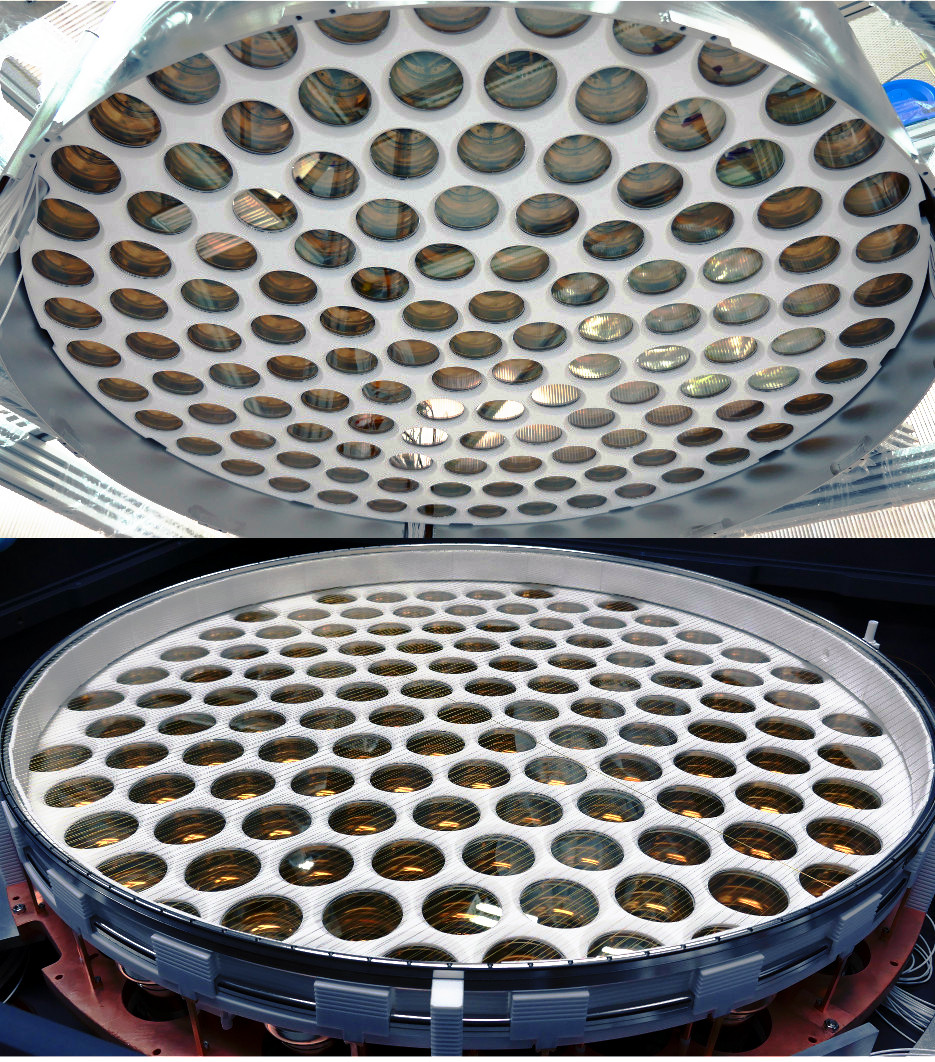
\includegraphics[width=0.5\textwidth]{figures/xe1t/pmt_arrays}
    \caption{Photograph of the arrays of R11410 photomultiplier tubes in XENON1T. (Top) The top 127 PMTs are arranged to optimize position reconstruction, while (bottom) the bottom 121 are optimized for light collection. The wires forming the cathode are barely visible above the bottom PMTs.}\label{fig:pmt_arrays}
\end{figure}

To determine the height of the liquid both inside and outside the bell, six capacitive levelmeters are installed. Four short levelmeters (SLM) measure the height of the liquid between the gate and anode, while two long levelmeters (LLM) measure the liquid level outside the TPC. The LLMs are of the concentric-cylinder variety, while the SLMs are formed from parallel plates.

The liquid level is set by pressurizing the bell through controlled xenon gas flow. The piping necessary for this, as well as the other pipes and cables for the PMTs, meshes, and other sensors, all run through an umbillical pipe and out the side of the water tank.